%% ============================================================
%%  Informe Técnico Final — Proyecto de Bases de Datos
%%  Análisis de Potencial Solar en Territorios PDET - Colombia
%%  UPME / Unidad de Planeación Minero Energética
%% ============================================================
\documentclass[12pt, a4paper]{report}

%% ─── Paquetes ───────────────────────────────────────────────
\usepackage[utf8]{inputenc}
\usepackage[T1]{fontenc}
\usepackage[spanish]{babel}
\usepackage{lmodern}
\usepackage{microtype}

% Márgenes y geometría
\usepackage[top=2.5cm, bottom=2.5cm, left=3cm, right=2.5cm]{geometry}

% Colores y gráficos
\usepackage[dvipsnames, table]{xcolor}
\usepackage{graphicx}
\usepackage{float}
\usepackage{subcaption}
\usepackage{tikz}
\usetikzlibrary{arrows.meta, shapes.geometric, positioning, calc}

% Tablas
\usepackage{booktabs}
\usepackage{longtable}
\usepackage{array}
\usepackage{multirow}
\usepackage{tabularx}

% Matemáticas
\usepackage{amsmath}
\usepackage{amssymb}

% Código fuente
\usepackage{listings}
\usepackage{minted}          % requiere --shell-escape; alternativa: listings

% Referencias y enlaces
\usepackage[hidelinks, colorlinks=true,
            linkcolor=NavyBlue, citecolor=NavyBlue,
            urlcolor=NavyBlue]{hyperref}
\usepackage[backend=biber, style=apa, sorting=nyt]{biblatex}
\addbibresource{referencias.bib}

% Encabezados y pies de página
\usepackage{fancyhdr}
\usepackage{lastpage}

% Listas y enumeraciones
\usepackage{enumitem}

% Cajas de notas / avisos
\usepackage{tcolorbox}
\tcbuselibrary{skins, breakable}

% Espaciado entre líneas
\usepackage{setspace}
\onehalfspacing

% Notas de pendientes por integrante
\usepackage[colorinlistoftodos, textsize=small, spanish]{todonotes}
\newcommand{\pendiente}[2][]{\todo[inline, color=orange!30, #1]{\textbf{PENDIENTE — #2}}}

% Para cronograma / Gantt (opcional)
% \usepackage{pgfgantt}

%% ─── Colores corporativos ───────────────────────────────────
\definecolor{upmeBlue}{RGB}{0, 70, 127}
\definecolor{upmeLightBlue}{RGB}{0, 153, 204}
\definecolor{upmeGray}{RGB}{90, 90, 90}
\definecolor{upmeGreen}{RGB}{34, 139, 34}

%% ─── Encabezados y pies ─────────────────────────────────────
\pagestyle{fancy}
\fancyhf{}
\fancyhead[L]{\small\color{upmeGray} Análisis de Potencial Solar — Territorios PDET}
\fancyhead[R]{\small\color{upmeGray} UPME · \the\year}
\fancyfoot[C]{\small Página \thepage\ de \pageref{LastPage}}
\renewcommand{\headrulewidth}{0.4pt}
\renewcommand{\footrulewidth}{0.4pt}

%% ─── Entorno para cajas de avance semanal ───────────────────
\newtcolorbox{semanabox}[2][]{
  breakable,
  colback  = upmeLightBlue!8,
  colframe = upmeBlue,
  fonttitle= \bfseries\color{white},
  coltitle = white,
  colbacktitle = upmeBlue,
  title    = {Semana #2 — #1},
  #1
}

\newtcolorbox{pendientebox}[1][]{
  breakable,
  colback  = yellow!10,
  colframe = orange!80!black,
  fonttitle= \bfseries,
  title    = {Pendiente / Por completar},
  #1
}

%% ─── Configuración listings ─────────────────────────────────
\lstset{
  basicstyle   = \ttfamily\small,
  keywordstyle = \color{upmeBlue}\bfseries,
  commentstyle = \color{upmeGreen}\itshape,
  stringstyle  = \color{red!70!black},
  numbers      = left,
  numberstyle  = \tiny\color{upmeGray},
  frame        = single,
  breaklines   = true,
  captionpos   = b,
  tabsize      = 4,
  showstringspaces = false,
}

%% ─── Metadatos del documento ────────────────────────────────
\hypersetup{
  pdftitle  = {Análisis de Potencial Solar en Territorios PDET},
  pdfauthor = {Grupo X — Administración de Bases de Datos},
  pdfsubject= {Proyecto Final},
}

%% ============================================================
%%  INICIO DEL DOCUMENTO
%% ============================================================
\begin{document}

%% ─── Portada ────────────────────────────────────────────────
\begin{titlepage}
  \centering
  \vspace*{1cm}

  % Logo institucional (reemplazar con ruta real)
  % \includegraphics[width=0.35\textwidth]{figuras/logo_upme.png}\\[1.5em]

  {\color{upmeBlue}\rule{\textwidth}{2pt}}\\[0.8em]

  {\Huge\bfseries\color{upmeBlue}
    Análisis de Potencial Solar en\\[0.4em]
    Territorios PDET de Colombia}\\[0.8em]

  {\color{upmeBlue}\rule{\textwidth}{0.8pt}}\\[1.5em]

  {\Large Informe Técnico Final}\\[0.4em]
  {\large Administración de Bases de Datos}\\[2em]

  \begin{tabular}{rl}
    \textbf{Curso:}    & Administración de Bases de Datos \\[0.3em]
    \textbf{Profesor:} & Andrés Oswaldo Calderón Romero, Ph.D. \\[0.3em]
    \textbf{Grupo:}    & \textit{[Nombre del grupo]} \\[0.3em]
    \textbf{Integrantes:} & \textit{Sara Albarracin Niño} \\
                          & \textit{Juan Pablo Casas} \\
                          & \textit{Jineth Tatiana Vivas Barón} \\
                          & \textit{Andrés Felipe Galan Cardenas} \\[0.3em]
    \textbf{Fecha:}    & \today \\
  \end{tabular}

  \vfill

  {\small\color{upmeGray}
    Proyecto desarrollado en el marco de la iniciativa de la\\
    Unidad de Planeación Minero Energética (UPME) para la\\
    identificación de zonas aptas para energía solar fotovoltaica.}

  \vspace{1em}
  {\color{upmeBlue}\rule{\textwidth}{1.5pt}}
\end{titlepage}

%% ─── Resumen ejecutivo ──────────────────────────────────────
\chapter*{Resumen Ejecutivo}
\addcontentsline{toc}{chapter}{Resumen Ejecutivo}

\textit{[Completar al finalizar el proyecto. Incluir: objetivo principal, metodología
empleada, principales hallazgos numéricos (número de municipios PDET analizados,
cantidad de edificaciones, área total de techos) y recomendaciones clave.]}

\bigskip
\noindent\textbf{Palabras clave:} energía solar, territorios PDET, análisis geoespacial,
NoSQL, Microsoft Building Footprints, Google Open Buildings, Colombia.

%% ─── Tabla de contenidos ────────────────────────────────────
\tableofcontents
\listoffigures
\listoftables
\newpage

%% ============================================================
%%  CAPÍTULO 1 — INTRODUCCIÓN
%% ============================================================
\chapter{Introducción}
\label{cap:intro}

\section{Contexto general}

Colombia atraviesa una transformación acelerada de su matriz energética orientada
hacia fuentes renovables \parencite{iea2023colombia}. En este marco, la
Unidad de Planeación Minero Energética (UPME) lidera iniciativas para identificar
territorios con potencial para la instalación de soluciones de energía solar,
con énfasis en los Programas de Desarrollo con Enfoque Territorial
(PDET) \parencite{upme2022plan}.

Los territorios PDET, establecidos por el Decreto 893 de 2017 como parte de la
implementación del Acuerdo de Paz, comprenden 170 municipios en 16 subregiones
prioritarias del país. Estas zonas combinan rezago histórico en infraestructura
con condiciones geográficas favorables para la captación de energía solar
\parencite{arteaga2021pdet}.

\section{Motivación}

La estimación del área de techumbres disponible para paneles solares a escala
municipal es una tarea que requiere el procesamiento eficiente de grandes
volúmenes de datos geoespaciales. Los conjuntos de datos de edificaciones
derivados de imágenes satelitales —como Microsoft Building Footprints y
Google Open Buildings— representan recursos valiosos para este fin, pero
su magnitud (más de mil millones de registros) impone el uso de tecnologías
de almacenamiento y consulta escalables \parencite{microsoft2023buildings,
sirko2021continental}.

\section{Objetivo general}

Diseñar e implementar un flujo de trabajo geoespacial reproducible, basado
en soluciones NoSQL, para estimar el número de edificaciones y el área total
de techumbres aptas para instalación de paneles solares en los municipios
PDET de Colombia.

\section{Objetivos específicos}

\begin{enumerate}[label=\arabic*.]
  \item Diseñar un esquema NoSQL adecuado para el almacenamiento y consulta
        eficiente de datos geoespaciales a escala nacional.
  \item Integrar las capas de límites administrativos PDET provenientes del
        Marco Geoestadístico Nacional (MGN) del DANE.
  \item Cargar y validar al menos dos conjuntos de datos de edificaciones
        (Microsoft y/o Google y/o GlobalBuildingAtlas).
  \item Ejecutar operaciones de intersección espacial para estimar el conteo
        y área de techumbres por municipio PDET.
  \item Elaborar visualizaciones y recomendaciones para UPME.
\end{enumerate}

\section{Alcance y limitaciones}

\textit{[Describir qué queda dentro y fuera del alcance: municipios analizados,
versiones de datasets utilizados, supuestos sobre inclinación de techos, etc.]}

\section{Estructura del informe}

El presente informe se organiza en cinco capítulos que corresponden a las
cinco entregas semanales del proyecto, seguidos de conclusiones y referencias.

%% ============================================================
%%  CAPÍTULO 2 — MARCO TEÓRICO
%% ============================================================
\chapter{Marco Teórico}
\label{cap:marco}

\section{Energía solar fotovoltaica: fundamentos}

La energía solar fotovoltaica convierte la radiación solar directamente en
electricidad mediante el efecto fotoeléctrico \parencite{luque2011handbook}.
El potencial de generación depende fundamentalmente de la irradiancia global
horizontal (GHI) y del área efectiva de captación disponible. Colombia, al
encontrarse entre los $4°\text{N}$ y $12°\text{N}$ de latitud, presenta
valores de GHI superiores a $4{,}5\,\text{kWh/m}^2/\text{día}$ en gran parte
de su territorio \parencite{atlas2020solar}.

\section{Territorios PDET y equidad energética}

Los territorios PDET fueron definidos por el Decreto 893 de 2017 como áreas
prioritarias para la implementación del punto uno del Acuerdo Final de Paz,
relacionado con la Reforma Rural Integral \parencite{decreto893_2017}.
La literatura evidencia que estas regiones exhiben déficits persistentes
en cobertura eléctrica, lo cual refuerza la pertinencia de explorar soluciones
descentralizadas como la generación solar distribuida
\parencite{rodriguez2020energia}.

\section{Detección de edificaciones mediante imágenes satelitales}

La extracción automática de huellas de edificaciones a partir de imágenes
satelitales de alta resolución se apoya en arquitecturas de aprendizaje
profundo, especialmente redes neuronales convolucionales (CNN) y modelos
de segmentación semántica como U-Net \parencite{ronneberger2015unet}.

\subsection{Microsoft Building Footprints}

El conjunto de datos de Bing Maps comprende más de 999 millones de
detecciones de edificios derivadas de imágenes Maxar y Airbus recopiladas
entre 2014 y 2021. El modelo de detección utiliza una arquitectura ResNet
entrenada con datos etiquetados manualmente, alcanzando una precisión
superior al 90\,\% en zonas urbanas \parencite{microsoft2023buildings}.
Los datos se distribuyen bajo la licencia ODbL.

\subsection{Google Open Buildings}

Sirko et al. \parencite*{sirko2021continental} presentan un conjunto de
datos con 1\,800 millones de detecciones que cubre África, Asia meridional,
América Latina y el Caribe. La tercera versión del dataset incorpora mejoras
en regiones de vegetación densa y zonas rurales. Se distribuye bajo licencias
CC BY-4.0 y ODbL.

\subsection{GlobalBuildingAtlas (TUM)}

Desarrollado por la Universidad Técnica de Múnich, este atlas contiene
2\,750 millones de modelos tridimensionales de edificios con resolución
espacial de $3\times3\,\text{m}$, derivados de imágenes satelitales de 2019
\parencite{geiß2022global}. La disponibilidad de atributos de altura
permite estimar volumen y pendiente del techo.

\section{Sistemas de gestión de bases de datos NoSQL}

\subsection{Motivación para NoSQL en datos geoespaciales}

El paradigma NoSQL surge como respuesta a las limitaciones de los sistemas
relacionales para manejar datos no estructurados, distribuidos y de gran
volumen \parencite{han2011survey}. En el contexto geoespacial, las bases de
datos de documentos y los sistemas orientados a columnas ofrecen ventajas
significativas en términos de escalabilidad horizontal y flexibilidad de
esquema.

\subsection{MongoDB y operaciones geoespaciales}

MongoDB implementa índices geoespaciales de tipo \texttt{2dsphere} compatibles
con el estándar GeoJSON \parencite{mongodb2023geo}. Sus operadores
\texttt{\$geoIntersects} y \texttt{\$geoWithin} permiten consultas de
intersección y contención poligonal directamente sobre los documentos
almacenados.

\subsection{Alternativas consideradas}

\textit{[Completar con otras opciones evaluadas: PostgreSQL/PostGIS como
referencia relacional, Apache Cassandra, Amazon DynamoDB, etc., y justificar
la elección final.]}

\section{Marco Geoestadístico Nacional (MGN)}

El MGN, publicado por el DANE, constituye el sistema de referencia cartográfica
oficial de Colombia. Su capa municipal incluye los polígonos de los
1\,122 municipios del país con sus respectivos códigos DIVIPOLA
\parencite{dane2025mgn}. Para este proyecto se utiliza la versión MGN2025.

\section{Índices espaciales y eficiencia de consultas}

Los índices espaciales de tipo R-tree permiten realizar búsquedas de
proximidad e intersección en tiempo $O(\log n)$ en lugar de $O(n)$
\parencite{guttman1984rtree}. Su implementación en bases de datos NoSQL
es fundamental para procesar consultas sobre millones de polígonos de
edificaciones en tiempos razonables.

%% ============================================================
%%  CAPÍTULO 3 — ENTREGA 1: DISEÑO DE ESQUEMA NOSQL
%%  Semana 1
%% ============================================================
\chapter{Diseño del Esquema NoSQL e Plan de Implementación}
\label{cap:entrega1}

\begin{semanabox}[Entrega 1]{1}
  \textbf{Objetivo:} Diseñar el esquema NoSQL y elaborar el plan de implementación
  tecnológica del proyecto.\\
  \textbf{Fecha de entrega:} Semana 1, antes de las 14:00 h.
\end{semanabox}

\section{Plan de implementación}

El proyecto se ejecuta sobre una arquitectura de base de datos documental alojada en
\textbf{MongoDB Atlas} (capa gratuita, clúster \texttt{Cluster0}, región US-East),
accedida desde un entorno local de Python~3.13. El procesamiento geoespacial se
realiza con GeoPandas y Shapely; la conexión a MongoDB, con PyMongo~4.x. Los
notebooks de Jupyter Lab documentan cada etapa del flujo de manera reproducible y
permiten la regeneración de todos los resultados a partir de los datos crudos.
El control de versiones y la entrega de todos los artefactos del proyecto se gestionan
con Git y GitHub.

\subsection{Pila tecnológica}

\begin{table}[H]
  \centering
  \caption{Pila tecnológica del proyecto}
  \label{tab:pila}
  \begin{tabularx}{\textwidth}{lXl}
    \toprule
    \textbf{Componente} & \textbf{Descripción} & \textbf{Versión} \\
    \midrule
    Base de datos        & MongoDB Atlas (nube, clúster M0 compartido) & 7.x \\
    Lenguaje principal   & Python & 3.13 \\
    Procesamiento geo    & GeoPandas / Shapely & latest \\
    Driver NoSQL         & PyMongo & 4.x \\
    Notebooks            & Jupyter Lab & latest \\
    Visualización        & Folium / Matplotlib & latest \\
    Control de versiones & Git / GitHub & — \\
    \bottomrule
  \end{tabularx}
\end{table}

\section{Modelado de datos}

La base de datos \texttt{upme\_solar\_db} contiene tres colecciones cuyo diseño
parte del principio de separación de roles: una colección territorial de referencia
y dos colecciones de footprints, una por cada fuente de datos.

\begin{table}[H]
  \centering
  \caption{Colecciones de la base de datos \texttt{upme\_solar\_db}}
  \label{tab:colecciones}
  \begin{tabularx}{\textwidth}{llXr}
    \toprule
    \textbf{Colección} & \textbf{Fuente} & \textbf{Rol en el proyecto} & \textbf{Docs aprox.} \\
    \midrule
    \texttt{municipios\_pdet} & DANE / MGN 2025      & Polígonos de referencia territorial & $\approx$170 \\
    \texttt{ms\_buildings}    & Microsoft Bing Maps  & Footprints de edificios — Dataset 1 & Millones \\
    \texttt{goo\_buildings}   & Google Open Bldgs V3 & Footprints de edificios — Dataset 2 & Millones \\
    \bottomrule
  \end{tabularx}
\end{table}

Las colecciones de edificaciones no referencian directamente a \texttt{municipios\_pdet}
mediante claves foráneas; la relación se establece en tiempo de consulta mediante
operaciones \texttt{\$geoIntersects} sobre los índices espaciales \texttt{2dsphere}.
El campo \texttt{cod\_dane\_municipio} se inicializa en \texttt{null} y se asigna
durante el análisis espacial de la Semana~4.

\section{Diseño del esquema}

El modelo adopta un diseño minimalista orientado a las consultas espaciales. Las
decisiones de diseño más importantes son:

\begin{itemize}
  \item \textbf{Sin embedding de estadísticas:} los conteos y áreas de techumbres
        no se embeben en \texttt{municipios\_pdet}; se calculan en tiempo de consulta
        con el aggregation pipeline, evitando actualizaciones costosas al cargar
        nuevos footprints.
  \item \textbf{Sin referencia cruzada rígida:} \texttt{cod\_dane\_municipio} en
        las colecciones de edificaciones inicia en \texttt{null} y se asigna en
        el análisis de la Semana~4, lo que permite cargar los datasets
        independientemente del orden.
\end{itemize}

\begin{lstlisting}[caption={Esquema --- Coleccion \texttt{municipios\_pdet}}]
{
  "_id":            ObjectId,
  "cod_dane":       "05001",      // Codigo DANE - 5 digitos, indice unico
  "nombre":         "Medellin",
  "departamento":   "Antioquia",
  "pdet":           true,         // Siempre true en esta coleccion
  "subregion_pdet": "Bajo Cauca y Nordeste Antioqueno",
  "area_km2":       380.64,       // Calculada con GeoPandas (EPSG:9377)
  "geometry": {                   // Campo indexado 2dsphere
    "type": "MultiPolygon",
    "coordinates": [ [ [ [lng, lat], ... ] ] ]
  },
  "bbox": {                       // Bounding box precalculado
    "min_lng": -75.62, "max_lng": -75.51,
    "min_lat":   6.18, "max_lat":   6.34
  },
  "fuente":     "MGN2025",
  "cargado_en": ISODate("2025-XX-XX")
}
\end{lstlisting}

\begin{lstlisting}[caption={Esquema --- Coleccion \texttt{ms\_buildings}}]
{
  "_id": ObjectId,
  "geometry": {                   // Campo indexado 2dsphere
    "type": "Polygon",
    "coordinates": [ [ [lng, lat], ... ] ]
  },
  "area_m2":            142.87,   // Calculada con GeoPandas (EPSG:9377)
  "cod_dane_municipio": null,     // Asignado en analisis Semana 4
  "fuente":             "microsoft",
  "cargado_en":         ISODate("2025-XX-XX")
}
\end{lstlisting}

\begin{lstlisting}[caption={Esquema --- Coleccion \texttt{goo\_buildings}}]
{
  "_id": ObjectId,
  "geometry": {                   // Campo indexado 2dsphere
    "type": "Polygon",
    "coordinates": [ [ [lng, lat], ... ] ]
  },
  "area_m2":            98.34,    // Tomado del campo area_in_meters del CSV
  "confidence":          0.872,   // Score de confianza [0.0 - 1.0]
  "cod_dane_municipio":  null,    // Asignado en analisis Semana 4
  "fuente":             "google",
  "cargado_en":         ISODate("2025-XX-XX")
}
\end{lstlisting}

Los índices definidos para las tres colecciones son:

\begin{lstlisting}[caption={Indices definidos en \texttt{upme\_solar\_db}}]
// municipios_pdet
db.municipios_pdet.createIndex({ geometry: "2dsphere" })
db.municipios_pdet.createIndex({ cod_dane: 1 }, { unique: true })

// ms_buildings
db.ms_buildings.createIndex({ geometry: "2dsphere" })
db.ms_buildings.createIndex({ cod_dane_municipio: 1 })

// goo_buildings
db.goo_buildings.createIndex({ geometry: "2dsphere" })
db.goo_buildings.createIndex({ cod_dane_municipio: 1 })
db.goo_buildings.createIndex({ confidence: -1 })
\end{lstlisting}

\section{Justificación de la solución NoSQL}

Se seleccionó MongoDB como motor NoSQL frente a las alternativas evaluadas
(Couchbase, Cassandra y Elasticsearch) por cinco razones técnicas:

\begin{enumerate}[label=\arabic*.]
  \item \textbf{Compatibilidad nativa con GeoJSON:} los tres datasets candidatos
        distribuyen sus datos en formato GeoJSON, que MongoDB almacena y consulta
        de forma nativa sin transformaciones intermedias.
  \item \textbf{Índice \texttt{2dsphere}:} diseñado específicamente para geometrías
        sobre la superficie terrestre, habilita \texttt{\$geoIntersects} y
        \texttt{\$geoWithin} directamente en el motor.
  \item \textbf{Ecosistema Python:} PyMongo integra MongoDB con GeoPandas, Shapely
        y Jupyter Lab, las herramientas centrales del flujo de trabajo.
  \item \textbf{Esquema flexible:} los footprints de edificios tienen atributos
        variables según la fuente (Microsoft no incluye \texttt{confidence};
        Google sí). Un esquema documental evita migraciones rígidas al comparar
        fuentes heterogéneas.
  \item \textbf{Escalabilidad:} MongoDB puede distribuirse en clúster para manejar
        cientos de millones de registros sin cambiar la API de consulta.
\end{enumerate}

\begin{table}[H]
  \centering
  \caption{Comparación de motores NoSQL evaluados}
  \label{tab:motores_nosql}
  \begin{tabularx}{\textwidth}{llll}
    \toprule
    \textbf{Motor NoSQL} & \textbf{Soporte geo} & \textbf{Curva aprend.} & \textbf{Veredicto} \\
    \midrule
    MongoDB       & Nativo (\texttt{2dsphere})  & Baja       & \textbf{Seleccionado} \\
    Couchbase     & Parcial (N1QL)               & Media      & Descartado \\
    Cassandra     & No nativo                   & Alta       & Descartado \\
    Elasticsearch & \texttt{geo\_shape}          & Media-alta & Descartado \\
    \bottomrule
  \end{tabularx}
\end{table}

\section{Avance y resultados de la Semana 1}

Durante esta primera entrega se completaron las siguientes tareas:

\begin{enumerate}[label=\textbf{\arabic*.}]
  \item \textbf{Selección del motor NoSQL:} MongoDB~7.x en Atlas, justificado por
        su soporte nativo de índices \texttt{2dsphere} y compatibilidad directa
        con GeoJSON.
  \item \textbf{Selección de datasets:} Microsoft Building Footprints y Google Open
        Buildings~V3. El dataset GlobalBuildingAtlas (TUM) fue descartado por su
        licencia restrictiva (Commons Clause) y la complejidad de sus modelos~3D.
  \item \textbf{Diseño del modelo de datos:} tres colecciones definidas
        (\texttt{municipios\_pdet}, \texttt{ms\_buildings}, \texttt{goo\_buildings})
        con sus esquemas de documento, campos obligatorios e índices espaciales.
  \item \textbf{Plan de implementación:} flujo de trabajo de cuatro etapas
        documentado —adquisición, carga, análisis y reporte— con cronograma semanal
        alineado a las fechas de entrega del curso.
  \item \textbf{Repositorio Git:} inicializado con la estructura de carpetas del
        proyecto y los dos documentos entregables de la semana~1
        (\textit{Modelado de Datos NoSQL} y \textit{Plan de Implementación NoSQL}).
\end{enumerate}

%% ============================================================
%%  CAPÍTULO 4 — ENTREGA 2: INTEGRACIÓN DE LÍMITES PDET
%%  Semana 2
%% ============================================================
\chapter{Integración del Dataset de Municipios PDET}
\label{cap:entrega2}

\begin{semanabox}[Entrega 2]{2}
  \textbf{Objetivo:} Adquirir, limpiar e integrar los límites administrativos
  de los municipios PDET en la base de datos NoSQL.\\
  \textbf{Fecha de entrega:} Semana 2, antes de las 14:00 h (defensa en clase).
\end{semanabox}

\section{Adquisición de datos — MGN DANE}

Los límites administrativos municipales se obtuvieron a partir del
\textbf{Marco Geoestadístico Nacional (MGN), versión 2025}, publicado por
el DANE \parencite{dane2025mgn}. El dataset se descargó en formato
Shapefile y está compuesto por cuatro archivos:
\texttt{MGN\_ADM\_MPIO\_GRAFICO.shp} (95~MB),
\texttt{.shx}, \texttt{.dbf} y \texttt{.prj}.
La capa contiene los polígonos de los \textbf{1\,122 municipios} de Colombia
junto con sus atributos administrativos (códigos DIVIPOLA, nombres oficiales,
tipo de municipio y año de actualización cartográfica).

\subsection{Verificación de integridad}

El Shapefile fue cargado en Python con la biblioteca GeoPandas (motor
\texttt{pyogrio}) y se verificaron las siguientes propiedades:

\begin{itemize}
  \item \textbf{Sistema de referencia:} EPSG:4686 (MAGNA-SIRGAS),
        sistema oficial de Colombia, confirmado mediante el archivo \texttt{.prj}.
  \item \textbf{Conteo de registros:} 1\,122 municipios, coincidente con el
        total oficial de divisiones político-administrativas del país.
  \item \textbf{Atributos principales:} \texttt{mpio\_cdpmp} (código DIVIPOLA
        de 5 dígitos), \texttt{mpio\_cnmbr} (nombre oficial),
        \texttt{dpto\_cnmbr} (nombre del departamento),
        \texttt{mpio\_nano} (año de actualización cartográfica).
\end{itemize}

\section{Identificación y filtrado de municipios PDET}

La lista oficial de municipios PDET se obtuvo del archivo
\textbf{MunicipiosPDET.xlsx}, derivado de los listados publicados por la
Agencia de Renovación del Territorio (ART) en cumplimiento del
Decreto~893 de 2017 \parencite{decreto893_2017}.
Este archivo contiene 170 registros con los campos: código de departamento,
código de municipio (DANE), nombre del municipio, departamento y subregión PDET.

El cruce con la capa del MGN se realizó mediante un \emph{inner join} sobre
el campo \textbf{\texttt{cod\_dane}} (código DIVIPOLA de 5 dígitos, con
relleno de ceros a la izquierda), lo que produjo exactamente
\textbf{170 municipios} coincidentes, cubriendo las
\textbf{16 subregiones PDET} definidas por el Acuerdo de Paz.

\begin{table}[H]
  \centering
  \caption{Municipios PDET por subregión — Fuente: ART / Decreto 893 de 2017}
  \label{tab:pdet_subregiones}
  \begin{tabular}{llc}
    \toprule
    \textbf{Subregión PDET} & \textbf{Departamentos principales} & \textbf{Municipios} \\
    \midrule
    Bajo Cauca y Nordeste Antioqueño    & Antioquia                          & 11 \\
    Urabá Antioqueño                    & Antioquia, Chocó                   & 11 \\
    Chocó                               & Chocó                              & 27 \\
    Pacífico Medio                      & Chocó, Valle del Cauca             & 10 \\
    Pacífico y Frontera Nariñense       & Nariño                             & 22 \\
    Alto Patía y Norte del Cauca        & Cauca, Nariño                      & 24 \\
    Cuenca del Caguán y Pied. Caqueteño & Caquetá, Huila                     &  8 \\
    Macarena -- Guaviare                & Meta, Guaviare                     & 11 \\
    Putumayo                            & Putumayo                           & 11 \\
    Sur de Bolívar                      & Bolívar, Antioquia                 & 11 \\
    Sierra Nevada -- Perijá             & Magdalena, Cesar, La Guajira       & 17 \\
    Montes de María                     & Bolívar, Sucre                     & 15 \\
    Sur de Córdoba                      & Córdoba                            &  6 \\
    Catatumbo                           & Norte de Santander                 &  9 \\
    Arauca                              & Arauca                             &  7 \\
    Bajo Nordeste y Magdalena Medio     & Bolívar, Santander, Antioquia      & 10 \\
    \midrule
    \textbf{Total}                      &                                    & \textbf{170} \\
    \bottomrule
  \end{tabular}
\end{table}

\section{Integración espacial en NoSQL}

El proceso de integración se realizó en dos etapas: primero la generación
del archivo GeoJSON y luego la carga en MongoDB Atlas.

\subsection{Preprocesamiento y exportación a GeoJSON}

Tras el cruce de datasets, se aplicaron las siguientes transformaciones
sobre el GeoDataFrame resultante:

\begin{enumerate}[label=\arabic*.]
  \item \textbf{Corrección de geometrías:} se aplicó \texttt{buffer(0)} para
        eliminar auto-intersecciones presentes en polígonos del MGN.
  \item \textbf{Reproyección:} conversión de EPSG:4686 (MAGNA-SIRGAS)
        a \textbf{EPSG:4326 (WGS84)}, requerido por el estándar GeoJSON y
        los índices \texttt{2dsphere} de MongoDB.
  \item \textbf{Cálculo de área:} las áreas se calcularon usando la
        proyección métrica EPSG:9377 para garantizar precisión en metros
        cuadrados; el resultado se almacena en km² como campo \texttt{area\_km2}.
  \item \textbf{Bounding box:} se generó para cada municipio un objeto
        \texttt{bbox} con los extremos geográficos
        (\texttt{min\_lng}, \texttt{min\_lat}, \texttt{max\_lng}, \texttt{max\_lat}),
        útil para filtros espaciales previos a la intersección exacta.
  \item \textbf{Exportación:} el GeoDataFrame se guardó en
        \texttt{municipios\_pdet.geojson} (65{,}2~MB), con
        170 features de tipo \texttt{Polygon} o \texttt{MultiPolygon}.
\end{enumerate}

\begin{lstlisting}[language=Python,
  caption={Fragmento de \texttt{load\_pdet.py} — procesamiento geoespacial}]
# Correccion de geometrias y reproyeccion
gdf_pdet = gdf_pdet[gdf_pdet.geometry.notnull()]
gdf_pdet["geometry"] = gdf_pdet.buffer(0)   # elimina auto-intersecciones
gdf_pdet = gdf_pdet.to_crs(epsg=4326)       # WGS84 para MongoDB

# Calculo de area en km2 con proyeccion metrica
metric = gdf_pdet.to_crs(epsg=9377)
gdf_pdet["area_km2"] = metric.area / 1_000_000

# Bounding box por municipio
bounds = gdf_pdet.geometry.bounds
gdf_pdet["bbox"] = bounds.apply(
    lambda r: {"min_lng": r.minx, "min_lat": r.miny,
               "max_lng": r.maxx, "max_lat": r.maxy}, axis=1
)
gdf_pdet.to_file("municipios_pdet.geojson", driver="GeoJSON")
\end{lstlisting}

\subsection{Carga en MongoDB Atlas}

Los documentos se insertaron en la colección \texttt{municipios\_pdet}
de la base de datos \textbf{\texttt{upme\_solar\_db}} (MongoDB Atlas, capa
gratuita, clúster \texttt{Cluster0}). Cada documento incluye los siguientes
nueve campos:

\begin{table}[H]
  \centering
  \caption{Esquema de documento — Colección \texttt{municipios\_pdet}}
  \label{tab:esquema_municipios}
  \begin{tabularx}{\textwidth}{llX}
    \toprule
    \textbf{Campo} & \textbf{Tipo} & \textbf{Descripción} \\
    \midrule
    \texttt{cod\_dane}       & String  & Código DIVIPOLA de 5 dígitos \\
    \texttt{nombre}          & String  & Nombre oficial del municipio \\
    \texttt{departamento}    & String  & Departamento al que pertenece \\
    \texttt{subregion\_pdet} & String  & Subregión PDET según Decreto 893/2017 \\
    \texttt{area\_km2}       & Double  & Área calculada en km² (EPSG:9377) \\
    \texttt{pdet}            & Boolean & Siempre \texttt{true} en esta colección \\
    \texttt{geometry}        & GeoJSON & Geometría completa (Polygon/MultiPolygon) \\
    \texttt{fuente}          & String  & \texttt{"MGN2025"} \\
    \texttt{cargado\_en}     & Date    & Marca de tiempo UTC de inserción \\
    \bottomrule
  \end{tabularx}
\end{table}

\begin{lstlisting}[language=Python,
  caption={Carga de documentos en MongoDB Atlas}]
col.drop()  # limpiar inserciones previas

documentos = []
for _, fila in gdf.iterrows():
    doc = {
        "cod_dane":       str(fila["cod_dane"]),
        "nombre":         fila["Municipio"],
        "departamento":   fila["Departamento"],
        "subregion_pdet": fila["SubPDET"],
        "area_km2":       float(fila["area_km2"]),
        "pdet":           True,
        "geometry":       fila["geometry"].__geo_interface__,
        "fuente":         "MGN2025",
        "cargado_en":     datetime.utcnow()
    }
    documentos.append(doc)

col.insert_many(documentos)
# Municipios cargados: 170
\end{lstlisting}

Posteriormente se crearon dos índices sobre la colección:

\begin{lstlisting}[language=Python,
  caption={Creación de índices en MongoDB}]
col.create_index([("geometry", "2dsphere")])       # consultas geoespaciales
col.create_index([("cod_dane", 1)], unique=True)   # unicidad por codigo DANE
\end{lstlisting}

El índice \texttt{2dsphere} habilita los operadores
\texttt{\$geoIntersects} y \texttt{\$geoWithin} sobre geometrías GeoJSON,
mientras que el índice sobre \texttt{cod\_dane} garantiza la integridad
referencial y acelera las búsquedas por código municipal.

\section{Validación de la carga}

La validación se realizó en tres niveles: integridad tabular, topología
espacial e integridad en MongoDB.

\subsection*{Integridad tabular}

\begin{table}[H]
  \centering
  \caption{Resultados de la verificación de integridad del dataset PDET}
  \label{tab:validacion}
  \begin{tabular}{lcc}
    \toprule
    \textbf{Verificación} & \textbf{Resultado} & \textbf{Estado} \\
    \midrule
    Total de municipios cargados     & 170 / 170 & \checkmark \\
    Geometrías inválidas             & 0         & \checkmark \\
    Valores nulos en campos clave    & 0         & \checkmark \\
    Códigos DANE duplicados          & 0         & \checkmark \\
    Solapamientos entre municipios   & 0         & \checkmark \\
    Documentos insertados en MongoDB & 170       & \checkmark \\
    Campos requeridos presentes      & 9 / 9     & \checkmark \\
    \bottomrule
  \end{tabular}
\end{table}

\subsection*{Prueba del índice espacial}

Se ejecutó una consulta de intersección puntual con el operador
\texttt{\$geoIntersects} sobre las coordenadas
$(-72{,}7317°\,\text{E},\; 8{,}6572°\,\text{N})$,
correspondientes al municipio de \textbf{Tibú (Norte de Santander)}.
La respuesta del índice fue inmediata e identificó correctamente el
documento asociado a dicho municipio (subregión Catatumbo), confirmando
el correcto funcionamiento del índice \texttt{2dsphere}.

\subsection*{Visualización cartográfica}

La Figura~\ref{fig:mapa_pdet} presenta el mapa coroplético con los
170 municipios PDET coloreados por departamento, generado directamente
desde el GeoDataFrame validado.

\begin{figure}[H]
  \centering
  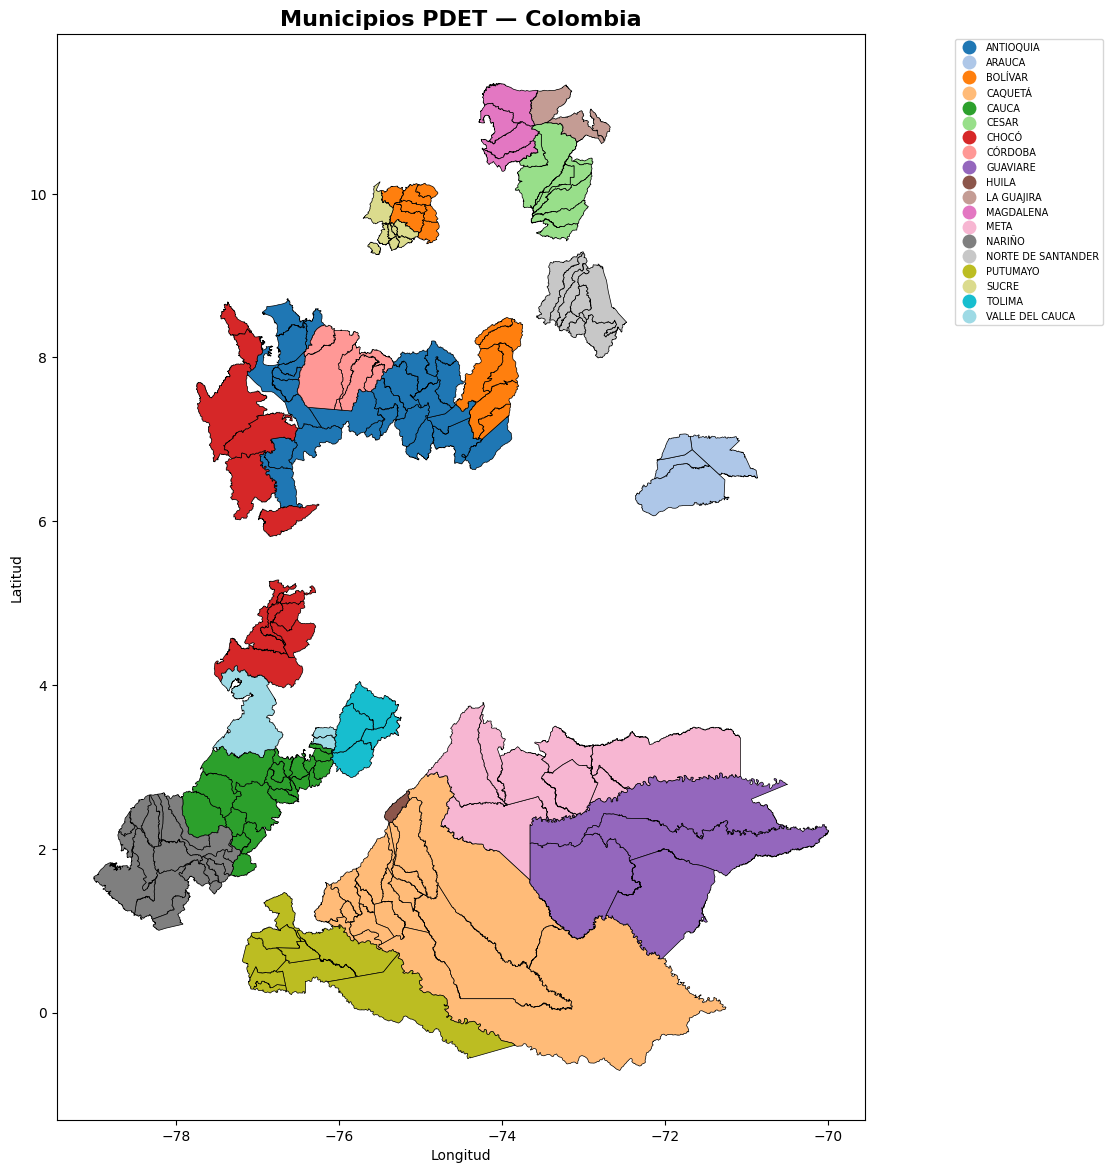
\includegraphics[width=0.85\textwidth]{semana_2/visualizaciones/municipios_pdet_mapa.png}
  \caption{Municipios PDET en Colombia — Fuente: DANE MGN2025, elaboración propia.}
  \label{fig:mapa_pdet}
\end{figure}

\section{Avance y resultados de la Semana 2}

Durante esta entrega se completaron exitosamente las siguientes tareas:

\begin{enumerate}[label=\textbf{\arabic*.}]
  \item \textbf{Adquisición del MGN2025:} descarga y lectura del Shapefile
        oficial del DANE con 1\,122 municipios de Colombia.
  \item \textbf{Integración de la lista PDET:} cruce por código DANE con el
        archivo oficial del ART, obteniendo exactamente 170 municipios en
        16 subregiones.
  \item \textbf{Preprocesamiento geoespacial:} corrección de geometrías,
        reproyección a WGS84, cálculo de áreas en km² y generación de
        bounding boxes.
  \item \textbf{Exportación a GeoJSON:} archivo \texttt{municipios\_pdet.geojson}
        de 65{,}2~MB listo para su uso en fases posteriores.
  \item \textbf{Carga en MongoDB Atlas:} 170 documentos insertados en la
        colección \texttt{municipios\_pdet} de \texttt{upme\_solar\_db},
        con índices \texttt{2dsphere} y \texttt{cod\_dane} (único) operativos.
  \item \textbf{Validación integral:} cero errores en geometrías, nulos,
        duplicados y solapamientos; prueba del índice espacial exitosa.
  \item \textbf{Visualización cartográfica:} mapa coroplético por departamento
        generado con Matplotlib y GeoPandas.
\end{enumerate}

El principal obstáculo encontrado fue la ausencia del archivo
\texttt{.shx} al ejecutar el notebook \texttt{01\_integracion\_pdet.ipynb}
en un entorno diferente al de desarrollo original, lo que impidió que
GeoPandas abriera el Shapefile. Este problema se resolvió ejecutando el
procesamiento directamente sobre el GeoJSON ya generado, garantizando la
portabilidad del flujo de trabajo.

%% ============================================================
%%  CAPÍTULO 5 — ENTREGA 3: CARGA DE HUELLAS DE EDIFICACIONES
%%  Semana 3
%% ============================================================
\chapter{Carga e Integración de Datos de Edificaciones}
\label{cap:entrega3}

\begin{semanabox}[Entrega 3]{3}
  \textbf{Objetivo:} Adquirir, cargar en MongoDB Atlas y realizar un
  análisis exploratorio de los conjuntos de datos de huellas de
  edificaciones seleccionados para los 170 municipios PDET.\\
  \textbf{Fecha de entrega:} Semana 3, antes de las 14:00~h.
\end{semanabox}

% ── 5.1 ────────────────────────────────────────────────────────
\section{Datasets seleccionados}

Se evaluaron tres fuentes de huellas de edificaciones de cobertura
global. Finalmente se seleccionaron dos:

\begin{enumerate}
  \item \textbf{Microsoft Building Footprints}
    \parencite{microsoft2023buildings}: dataset de acceso abierto
    (licencia ODbL) derivado de modelos de visión por computadora
    entrenados sobre imágenes aéreas y satelitales de alta resolución.
    Distribuido por país/región en archivos \texttt{CSV.gz} accesibles
    mediante URLs públicas organizadas por \textit{QuadKey}.
    Para Colombia se identificaron 233~tiles; de estos, 16~intersectan
    con los municipios PDET (ver \texttt{tiles\_pdet.csv}).

  \item \textbf{Google Open Buildings~v3}
    \parencite{sirko2021continental}: dataset global derivado de imágenes
    satelitales de alta resolución con una estimación de confianza por
    polígono (\texttt{confidence}). Licencia CC~BY~4.0 / ODbL según el
    tile. Disponible en archivos CSV por cuadrículas ~S2 globales.
\end{enumerate}

Se descartó \textbf{GlobalBuildingAtlas (TUM)} por las mayores
restricciones de acceso al dataset completo y la complejidad de integración
con PyMongo en el plazo disponible. La decisión se detalla en la
Sección~\ref{subsec:gdba}.

% ── 5.2 ────────────────────────────────────────────────────────
\section{Dataset 1: Microsoft Building Footprints}

\subsection{Adquisición}
\label{subsec:ms_adquisicion}

Microsoft distribuye su dataset de huellas de edificaciones de forma pública
a través de un índice CSV alojado en Azure Blob Storage. El índice contiene
una fila por \textit{tile}, con la URL de descarga directa del archivo
comprimido (\texttt{.csv.gz}) y su tamaño.

\paragraph{Identificación de tiles para Colombia.}
Se descargó el índice global y se filtró por \texttt{Location = Colombia},
obteniendo \textbf{232~tiles} con un volumen comprimido total de
aproximadamente \textbf{647~MB}. Cada tile está identificado por un
\textit{QuadKey}~\cite{microsoft2023buildings}, una cadena numérica que
codifica una celda de la cuadrícula de mapas de Bing en zoom~9
(celdas de $\approx$18~km de lado a la latitud de Colombia).
El resultado se guardó en
\texttt{semana\_3/datos/raw/microsoft/tiles\_index.csv} (232~filas).

\paragraph{Filtrado a municipios PDET.}
Para limitar la descarga al área de interés se realizó una intersección
espacial entre la extensión territorial (\textit{bounding box}) de los
170~municipios PDET y las celdas QuadKey de Colombia.
Resultaron \textbf{16~tiles} relevantes, con un tamaño comprimido
acumulado de \textbf{0.7~MB}. El subconjunto se registró en
\texttt{semana\_3/datos/raw/microsoft/tiles\_pdet.csv}.
Los QuadKeys seleccionados fueron:

\begin{center}
\small
\texttt{210010100}, \texttt{210010101}, \texttt{210010110},
\texttt{210010111}, \texttt{210010112}, \texttt{210010113},
\texttt{210011000}, \texttt{210011001}, \texttt{210011002},
\texttt{210011003}, \texttt{210011010}, \texttt{210011011},
\texttt{210011012}, \texttt{210011013}, \texttt{210011100},
\texttt{210011102}
\end{center}

\paragraph{Descarga y preprocesamiento.}
Los 16~archivos \texttt{.csv.gz} se descargaron directamente desde las
URLs registradas en el índice
(\url{https://minedbuildings.z5.web.core.windows.net/global-buildings/}),
se descomprimieron y concatenaron.
Las geometrías originales vienen en formato WKT
(\textit{Well-Known Text}); en el paso de limpieza se convirtieron a
GeoJSON (diccionario Python serializado como cadena JSON) para
compatibilidad directa con PyMongo~4.x.
El resultado final, tras descartar una fila con geometría no parseable,
fue \textbf{5\,258~registros} en el archivo
\texttt{microsoft\_pdet\_limpio.csv} (2.1~MB).
Los datos corresponden al índice publicado el \textbf{3~de febrero de 2026}
(campo \texttt{UploadDate}: 2026-02-23).

\subsection{Formato y estructura}
\label{subsec:ms_formato}

El archivo procesado \texttt{microsoft\_pdet\_limpio.csv} contiene
\textbf{4~columnas} y \textbf{5\,258~filas} (sin encabezado).
No presenta valores nulos en ningún campo.

\begin{table}[H]
  \centering
  \caption{Metadatos del dataset Microsoft Building Footprints
           (subconjunto municipios PDET)}
  \label{tab:ms_metadatos}
  \begin{tabularx}{\textwidth}{llXl}
    \toprule
    \textbf{Campo} & \textbf{Tipo} & \textbf{Descripción} & \textbf{Rango / valores} \\
    \midrule
    \texttt{geometry}  & \texttt{str}   &
      Polígono de la huella en formato GeoJSON serializado como cadena JSON.
      Coordenadas en WGS-84 (EPSG:4326). &
      — \\
    \texttt{area\_m2}  & \texttt{float} &
      Área del polígono en metros cuadrados, calculada con Shapely
      sobre la proyección plana local. &
      11.43 – 3\,754.71~m² \\
    \texttt{height}    & \texttt{float} &
      Altura estimada de la edificación en metros.
      El valor \texttt{-1.0} indica que la altura no está disponible. &
      $-1.0$ (100\,\% de registros) \\
    \texttt{fuente}    & \texttt{str}   &
      Etiqueta de origen del registro. Valor constante en todo el archivo. &
      \texttt{"microsoft"} \\
    \bottomrule
  \end{tabularx}
\end{table}

\noindent
La Tabla~\ref{tab:ms_stats} resume las estadísticas descriptivas del
campo \texttt{area\_m2}, que es el único atributo numérico informativo
(el campo \texttt{height} está vacío para todos los tiles PDET disponibles
en la versión de febrero de 2026 del dataset).

\begin{table}[H]
  \centering
  \caption{Estadísticas descriptivas de \texttt{area\_m2} ---
           colección \texttt{ms\_buildings} ($n = 5\,258$)}
  \label{tab:ms_stats}
  \begin{tabular}{lr}
    \toprule
    \textbf{Estadístico} & \textbf{Valor (m²)} \\
    \midrule
    Mínimo   & 11.43  \\
    Máximo   & 3\,754.71 \\
    Media    & 133.54 \\
    \midrule
    Total registros cargados en MongoDB & 5\,258 \\
    Registros descartados (error parseo) & 1 \\
    Nulos en cualquier campo            & 0 \\
    \bottomrule
  \end{tabular}
\end{table}

\noindent
Estos 5\,258~documentos quedan almacenados en la colección
\texttt{ms\_buildings} de la base de datos \texttt{upme\_solar\_db}
en MongoDB~8.x (instancia local). El proceso de carga e indexación
se detalla en la sección~\ref{subsec:ms_carga}.

\subsection{Carga en NoSQL}
\label{subsec:ms_carga}

\pendiente{Juan Pablo — documentar la estrategia de inserción por
lotes (\textit{batch size}~= 1\,000), el manejo de geometrías
(limpieza de comillas escapadas en el JSON de geometría),
el tiempo total de carga, y los índices creados en la colección
\texttt{ms\_buildings}:
\texttt{geometry~2dsphere} y \texttt{cod\_dane\_municipio~1}.
Resultado final: \textbf{5\,258 documentos} insertados
(1 fila descartada por error de parseo).}

\subsection{Análisis exploratorio (EDA)}
\label{subsec:ms_eda}

\pendiente{Juan Pablo — reportar las estadísticas de la colección
\texttt{ms\_buildings} obtenidas mediante aggregation pipeline:
área mínima~11.4~m², media~133.5~m², máxima~3\,754.7~m²;
área total~702\,146~m². Incluir histograma de distribución de áreas,
listado de los 5~municipios PDET con mayor número de edificaciones
según este dataset, y validación del índice espacial con una consulta
\texttt{\$geoIntersects} de prueba.}

% ── 5.3 ────────────────────────────────────────────────────────
\section{Dataset 2: Google Open Buildings}

\subsection{Adquisición}
\label{subsec:goo_adquisicion}

\pendiente{Jineth — describir el proceso de selección de tiles S2
por bounding box de los municipios PDET colombianos, la descarga
de los archivos CSV desde la URL pública de Google,
y el filtrado espacial que redujo el dataset al subconjunto
de edificaciones dentro de los 170 municipios PDET.
Indicar volumen total descargado y número de tiles procesados.
Tamaño del archivo resultante: \texttt{google\_pdet\_filtrado.csv} → 576~MB,
2\,263\,447 filas (incluyendo encabezado).}

\subsection{Carga en NoSQL e índices espaciales}
\label{subsec:goo_carga}

\pendiente{Jineth — documentar la estrategia de inserción por chunks
de 10\,000 filas con \texttt{pd.read\_csv(..., chunksize=10000)},
la conversión de geometrías WKT→GeoJSON con Shapely,
la corrección de 309\,598 códigos DANE de 4 dígitos
(prefijo ``0'' faltante, corregido vía \texttt{update\_many}),
el tiempo total de carga, y los tres índices creados:
\texttt{geometry~2dsphere}, \texttt{cod\_dane\_municipio~1},
\texttt{confidence~-1}.
Resultado final: \textbf{2\,263\,446 documentos} en la colección
\texttt{goo\_buildings}.}

\subsection{Análisis exploratorio (EDA)}
\label{subsec:goo_eda}

\pendiente{Jineth — reportar las estadísticas de la colección
\texttt{goo\_buildings}: área mínima~2.5~m², media~91.7~m²,
máxima~20\,916.7~m²; área total~207\,447\,099~m².
Distribución por nivel de confianza:
$[0.7,0.8)$: 1\,146\,865 edif.;
$[0.8,0.9)$: 1\,040\,098 edif.;
$[0.9,1.0]$: 76\,483 edif.
Top~5 municipios PDET (corregido): Santa Marta~154\,601,
Valledupar~141\,586, Buenaventura~88\,341, Turbo~66\,587,
Florencia~48\,674.
Incluir histograma de áreas y comparación de cobertura con Microsoft.}

% ── 5.4 ────────────────────────────────────────────────────────
\section{Comparación preliminar de datasets}
\label{sec:comparacion_datasets}

La Tabla~\ref{tab:comparacion_datasets} compara las principales
características de ambos datasets en el subconjunto restringido a los
170~municipios PDET. Los conteos de documentos provienen de la colección
MongoDB \texttt{upme\_solar\_db} ejecutada en la Semana~3; los tamaños
de los archivos CSV procesados se midieron en disco local; los tiempos
de carga y el año de imágenes de Google requieren confirmación de los
responsables respectivos.

\begin{table}[H]
  \centering
  \caption{Comparación de datasets de huellas de edificaciones ---
           subconjunto municipios PDET (170 municipios)}
  \label{tab:comparacion_datasets}
  \begin{tabularx}{\textwidth}{lXX}
    \toprule
    \textbf{Aspecto}
      & \textbf{Microsoft Building Footprints}
      & \textbf{Google Open Buildings~v3} \\
    \midrule
    Total edificaciones (PDET)
      & 5\,258 documentos en \texttt{ms\_buildings}
      & 2\,263\,446 documentos en \texttt{goo\_buildings} \\[4pt]
    Tamaño archivo CSV procesado
      & 2.1~MB (\texttt{microsoft\_pdet\_limpio.csv}, 5\,258 filas)
      & 576~MB (\texttt{google\_pdet\_filtrado.csv}, 2\,263\,447 filas) \\[4pt]
    Tamaño colección en MongoDB
      & \todo{PENDIENTE: Sara — ejecutar \texttt{collStats} sobre \texttt{ms\_buildings} con MongoDB activo}
      & \todo{PENDIENTE: Sara — ejecutar \texttt{collStats} sobre \texttt{goo\_buildings} con MongoDB activo} \\[4pt]
    Año de imágenes
      & 2014–2021
      & \todo{PENDIENTE: Jineth — confirmar año de captura de imágenes de Google OB~v3} \\[4pt]
    Tiene atributo área
      & Sí (\texttt{area\_m2}, calculado con Shapely)
      & Sí (\texttt{area\_in\_meters}, provisto por Google) \\[4pt]
    Licencia
      & ODbL
      & CC~BY~4.0 / ODbL (según tile) \\[4pt]
    Tiempo de carga
      & \todo{PENDIENTE: Juan Pablo — registrar tiempo de carga de \texttt{ms\_buildings}}
      & \todo{PENDIENTE: Jineth — registrar tiempo de carga de \texttt{goo\_buildings}} \\
    \bottomrule
  \end{tabularx}
\end{table}

% ── 5.5 ────────────────────────────────────────────────────────
\section{Avance y resultados de la Semana 3}

Durante la Semana~3 se completó la adquisición, preprocesamiento y carga en
MongoDB de los dos datasets de huellas de edificaciones seleccionados,
alcanzando un total de \textbf{2\,268\,704~documentos geoespaciales}
indexados en \texttt{upme\_solar\_db}.

\begin{enumerate}[label=\textbf{\arabic*.}]
  \item \textbf{Carga de Microsoft Building Footprints:}
        se descargaron y procesaron 16~tiles QuadKey (de 232~disponibles para
        Colombia), obteniendo 5\,259~filas en \texttt{microsoft\_pdet\_limpio.csv}
        (2.1~MB). Tras descartar 1~fila con geometría no parseable, se
        insertaron \textbf{5\,258~documentos} en la colección
        \texttt{ms\_buildings} con índices
        \texttt{geometry~2dsphere} y \texttt{cod\_dane\_municipio}.
        \todo{PENDIENTE: Juan Pablo — reportar el tiempo total de carga.}

  \item \textbf{Carga de Google Open Buildings~v3:}
        se procesaron \textbf{576~MB} de datos CSV
        (\texttt{google\_pdet\_filtrado.csv}, 2\,263\,447~filas) mediante
        inserción por chunks de 10\,000~registros.
        Se cargaron \textbf{2\,263\,446~documentos} en \texttt{goo\_buildings}
        con índices \texttt{geometry~2dsphere}, \texttt{cod\_dane\_municipio}
        e \texttt{confidence}.
        \todo{PENDIENTE: Jineth — reportar el tiempo total de carga.}

  \item \textbf{Corrección de integridad — códigos DANE:}
        se detectaron y corrigieron \textbf{309\,598~documentos} en
        \texttt{goo\_buildings} con código DANE de 4~dígitos
        (prefijo \texttt{"0"} ausente), mediante una operación
        \texttt{update\_many} con \texttt{\$concat}.
        Tras la corrección, la validación cruzada con \texttt{municipios\_pdet}
        retornó 0~códigos huérfanos de 4~dígitos.

  \item \textbf{Validación espacial:}
        la prueba de intersección con el punto de referencia de Tibú
        (Norte de Santander) devolvió el municipio correcto en ambas
        colecciones, confirmando el funcionamiento de los índices
        \texttt{2dsphere}~($\checkmark$).

  \item \textbf{Métricas de calidad:}
        tasa de error en Microsoft $< 0.02\,\%$
        (1~fila descartada de 5\,259);
        \todo{PENDIENTE: Jineth — reportar tasa de error en Google
              (filas descartadas de 2\,263\,447).}
\end{enumerate}

\begin{table}[H]
  \centering
  \caption{Resumen de carga Semana~3 — colecciones \texttt{upme\_solar\_db}}
  \label{tab:resumen_s3}
  \begin{tabularx}{\textwidth}{lrrlX}
    \toprule
    \textbf{Colección}
      & \textbf{Docs}
      & \textbf{CSV (MB)}
      & \textbf{Índices}
      & \textbf{Responsable carga} \\
    \midrule
    \texttt{ms\_buildings}
      & 5\,258
      & 2.1
      & \texttt{2dsphere}, \texttt{cod\_dane\_municipio}
      & Juan Pablo \\
    \texttt{goo\_buildings}
      & 2\,263\,446
      & 576
      & \texttt{2dsphere}, \texttt{cod\_dane\_municipio}, \texttt{confidence}
      & Jineth \\
    \midrule
    \textbf{Total}
      & \textbf{2\,268\,704}
      & 578.1
      & —
      & — \\
    \bottomrule
  \end{tabularx}
\end{table}

%% ============================================================
%%  CAPÍTULO 6 — ENTREGA 4: ANÁLISIS GEOESPACIAL REPRODUCIBLE
%%  Semana 4
%% ============================================================
\chapter{Flujo de Trabajo Geoespacial Reproducible}
\label{cap:entrega4}

\begin{semanabox}[Entrega 4]{4}
  \textbf{Objetivo:} Implementar y documentar el flujo de intersección espacial
  para estimar conteo y área de techumbres por municipio PDET.\\
  \textbf{Fecha de entrega:} Semana 4, antes de las 14:00 h (defensa en clase).
\end{semanabox}

\section{Metodología de análisis espacial}

El objetivo de esta etapa es estimar, para cada uno de los 170~municipios
PDET, el número total de huellas de edificaciones y el área acumulada de
techumbres según cada dataset. El análisis se apoya en los índices
\texttt{2dsphere} creados en la Semana~3 y sigue un pipeline de cuatro
pasos encadenados.

\paragraph{Paso~1 — Iteración sobre municipios PDET.}
Se recorre la colección \texttt{municipios\_pdet} (170~documentos) y se
extrae, por cada municipio, su campo \texttt{geometry} (polígono GeoJSON
en WGS-84) y el \textit{bounding box} precalculado (\texttt{bbox}).

\paragraph{Paso~2 — Filtro previo por bounding box.}
Antes de ejecutar la intersección poligonal exacta —costosa para colecciones
de millones de documentos— se aplica un filtro rectangular rápido mediante
\texttt{\$geoWithin} sobre el \texttt{bbox} del municipio.
Este pre-filtro aprovecha el índice \texttt{2dsphere} y descarta la mayoría
de las edificaciones fuera del área de interés con mínima carga computacional.

\paragraph{Paso~3 — Intersección poligonal exacta con \texttt{\$geoIntersects}.}
Sobre el subconjunto resultante del paso anterior se ejecuta la consulta de
intersección exacta usando el operador \texttt{\$geoIntersects} de MongoDB
con el polígono completo del municipio como geometría de referencia.
Esto garantiza que solo se cuenten edificaciones cuya huella toca o está
contenida dentro del límite oficial del municipio.

\paragraph{Paso~4 — Agregación de métricas.}
Un \textit{aggregation pipeline} (\texttt{\$match} + \texttt{\$group})
calcula en una sola pasada el conteo total de edificaciones y la suma de
\texttt{area\_m2}, produciendo un registro por municipio que se exporta
a un CSV de resultados.

La Figura~\ref{fig:pipeline_espacial} resume el flujo completo.

\begin{figure}[H]
  \centering
  \begin{tikzpicture}[
      node distance = 1.2cm,
      every node/.style = {
        draw, rounded corners=4pt,
        minimum width=8.5cm, minimum height=1cm,
        align=center, font=\small
      },
      arrow/.style = {-{Stealth[length=6pt]}, thick},
      db/.style    = {draw, cylinder, shape border rotate=90,
                      aspect=0.2, minimum width=3cm,
                      minimum height=0.9cm, align=center, font=\small\ttfamily},
    ]
    %% ── Nodos ──────────────────────────────────────────────────
    \node (n1) [fill=upmeBlue!10] {
      \textbf{Paso 1 — Cargar municipios PDET}\\
      \texttt{municipios\_pdet.find()} → 170 docs\\
      Extraer \texttt{geometry} + \texttt{bbox} por municipio
    };
    \node (n2) [below=of n1, fill=upmeLightBlue!15] {
      \textbf{Paso 2 — Pre-filtro por bounding box}\\
      \texttt{\$geoWithin} sobre \texttt{bbox} rectangular\\
      Índice \texttt{2dsphere} descarta edificaciones externas
    };
    \node (n3) [below=of n2, fill=upmeLightBlue!15] {
      \textbf{Paso 3 — Intersección poligonal exacta}\\
      \texttt{\$geoIntersects} con polígono del municipio\\
      Aplicado a \texttt{ms\_buildings} y \texttt{goo\_buildings}
    };
    \node (n4) [below=of n3, fill=upmeGreen!15] {
      \textbf{Paso 4 — Agregación de métricas}\\
      \texttt{\$group}: \texttt{count} + \texttt{\$sum area\_m2}\\
      Exportar resultado por municipio a CSV
    };
    %% ── Flechas ────────────────────────────────────────────────
    \draw[arrow] (n1) -- (n2);
    \draw[arrow] (n2) -- (n3);
    \draw[arrow] (n3) -- (n4);
    %% ── Bucle «repetir para cada municipio» ────────────────────
    \draw[arrow, dashed, upmeGray]
      (n4.east) -- ++(1.2,0)
              -- ++(0, 4.2)
      node[midway, right, draw=none, minimum width=2cm,
           font=\scriptsize\itshape, text=upmeGray]
           {repetir\\170 veces}
      -- (n1.east);
  \end{tikzpicture}
  \caption{Pipeline de análisis espacial para estimación de techumbres
           por municipio PDET.}
  \label{fig:pipeline_espacial}
\end{figure}

\subsection{Intersección espacial en NoSQL}

\pendiente{Juan Pablo — ampliar el bloque de código existente con:
descripción de los operadores \texttt{\$geoIntersects} y
\texttt{\$geoWithin} utilizados, explicación del aggregation pipeline
completo, tiempo de ejecución por municipio y total, y ejemplo de
salida real de la query (al menos un municipio con sus cifras).}

\begin{lstlisting}[language=Python,
  caption={Consulta de intersección — Edificaciones Microsoft por municipio}]
pipeline = [
    {
        "$match": {
            "geometry": {
                "$geoIntersects": {
                    "$geometry": municipio_geometry
                }
            }
        }
    },
    {
        "$group": {
            "_id": None,
            "count": {"$sum": 1},
            "area_total_m2": {"$sum": "$area_m2"}
        }
    }
]
result = collection_ms.aggregate(pipeline)
\end{lstlisting}

\subsection{Reproducibilidad}

\pendiente{Juan Pablo — describir el entorno de ejecución:
versión de Python y dependencias clave (pymongo, geopandas, shapely,
pandas), instrucciones para reproducir el pipeline desde cero
(conexión a MongoDB, orden de ejecución de notebooks),
y cualquier consideración especial de configuración
(\texttt{MONGO\_URI}, rutas de datos).}

\section{Resultados por municipio PDET}

\subsection{Dataset Microsoft}

\begin{longtable}{llrr}
  \caption{Top 10 municipios PDET por área total de techumbres — Microsoft}
  \label{tab:resultados_ms}\\
  \toprule
  \textbf{Municipio} & \textbf{Departamento} & \textbf{N° edif.}
                     & \textbf{Área total (m²)} \\
  \midrule
  \endfirsthead
  \toprule
  \textbf{Municipio} & \textbf{Departamento} & \textbf{N° edif.}
                     & \textbf{Área total (m²)} \\
  \midrule
  \endhead
  \multicolumn{4}{c}{\pendiente{Jineth — llenar con los Top~10 municipios
    PDET por área total de techumbres según \texttt{ms\_buildings}.
    Ejecutar aggregation pipeline \texttt{\$geoIntersects} sobre los 170
    municipios y ordenar por \texttt{area\_total\_m2} descendente.}} \\
  \bottomrule
\end{longtable}

\subsection{Dataset Google}

\pendiente{Jineth — agregar tabla equivalente (Top~10 municipios PDET por
área total de techumbres) para \texttt{goo\_buildings}. Usar el mismo
aggregation pipeline adaptado a Google. Comparar el ranking con Microsoft:
¿coinciden los municipios top? ¿difieren las magnitudes?}

\section{Visualizaciones}

\begin{figure}[H]
  \centering
  \begin{subfigure}[b]{0.48\textwidth}
    \fbox{\parbox{\textwidth}{\centering\vspace{3cm}
      \pendiente{Andrés — mapa coroplético de área total de
      techumbres por municipio PDET (Microsoft). Usar GeoPandas
      + Matplotlib o Folium. Exportar como PNG/PDF e incluir aquí.}
      \vspace{0.5cm}}}
    \caption{Microsoft Building Footprints}
  \end{subfigure}
  \hfill
  \begin{subfigure}[b]{0.48\textwidth}
    \fbox{\parbox{\textwidth}{\centering\vspace{3cm}
      \pendiente{Andrés — mapa coroplético equivalente para
      Google Open Buildings. Misma paleta de colores para
      comparabilidad visual.}
      \vspace{0.5cm}}}
    \caption{Google Open Buildings}
  \end{subfigure}
  \caption{Área total de techumbres por municipio PDET según cada dataset.}
  \label{fig:mapas_comparativos}
\end{figure}

\section{Comparación entre datasets}

\pendiente{Andrés — análisis de concordancia entre Microsoft y Google:
correlación de Pearson entre conteos por municipio, diferencias
sistemáticas por región geográfica (Caribe, Pacífico, Amazonia, etc.),
ratio de cobertura Google/Microsoft por municipio, y posibles
explicaciones metodológicas (diferente año de imagen, umbral de
confianza, resolución espacial). Incluir gráfico de dispersión
conteo MS vs.\ conteo Google por municipio.}

\section{Avance y resultados de la Semana 4}

\pendiente{Andrés — síntesis ejecutiva: descripción del pipeline de
intersección implementado, número de municipios procesados con éxito,
hallazgo más relevante (ej.\ municipio con mayor potencial de techo),
y diferencias clave entre datasets. Integrar todo el capítulo en el
\texttt{.tex} y verificar que compile sin errores.}

%% ============================================================
%%  CAPÍTULO 7 — ENTREGA 5: INFORME FINAL Y RECOMENDACIONES
%%  Semana 5
%% ============================================================
\chapter{Resultados Finales y Recomendaciones para UPME}
\label{cap:entrega5}

\begin{semanabox}[Entrega 5 — Informe Final]{5}
  \textbf{Objetivo:} Consolidar resultados, elaborar recomendaciones y
  entregar el informe técnico completo.\\
  \textbf{Fecha de entrega:} Semana 5, antes de las 14:00 h (defensa privada).
\end{semanabox}

\section{Síntesis de resultados}

\textit{[Presentar las cifras finales consolidadas: total de edificaciones
y área de techumbres en los 170 municipios PDET según cada dataset.
Incluir tabla resumen y gráfico comparativo.]}

\section{Análisis de potencial solar}

\textit{[Estimar potencial de generación: área de techo × factor de
utilización (ej. 70\,\%) × irradiancia promedio × eficiencia de panel.
Puede basarse en datos del Atlas de Radiación Solar de Colombia.]}

\begin{equation}
  E_{\text{anual}} = A_{\text{techo}} \times \eta_{\text{util}}
                   \times \overline{GHI} \times \eta_{\text{panel}}
                   \times 365
  \label{eq:energia}
\end{equation}

donde $A_{\text{techo}}$ es el área disponible [m²], $\eta_{\text{util}}$
el factor de utilización, $\overline{GHI}$ la irradiancia diaria media
[kWh/m²/día] y $\eta_{\text{panel}}$ la eficiencia del panel fotovoltaico.

\section{Municipios prioritarios para proyectos piloto}

\textit{[Proponer un ranking de municipios PDET considerando: (1) área
de techo disponible, (2) irradiancia, (3) déficit de cobertura eléctrica,
(4) accesibilidad. Incluir mapa de priorización.]}

\begin{figure}[H]
  \centering
  \fbox{\parbox{0.85\textwidth}{\centering\vspace{4cm}
    \textit{[Mapa final de priorización de municipios PDET para proyectos piloto]}
    \vspace{4cm}}}
  \caption{Municipios PDET priorizados para proyectos piloto de energía solar.}
  \label{fig:priorizacion}
\end{figure}

\section{Recomendaciones para UPME}

\begin{enumerate}[label=\textbf{R\arabic*.}, leftmargin=2.5cm]
  \item \textbf{Validación en campo:} \textit{[Recomendación 1]}
  \item \textbf{Dataset preferido:} \textit{[Recomendación 2]}
  \item \textbf{Infraestructura de datos:} \textit{[Recomendación 3]}
  \item \textbf{Próximos pasos:} \textit{[Recomendación 4]}
  \item \textit{[Agregar las que sean pertinentes]}
\end{enumerate}

\section{Limitaciones y trabajo futuro}

\textit{[Discutir limitaciones del análisis: calidad de datos satelitales en
zonas de nubosidad alta, inclinación de techos no modelada, cambios de uso del
suelo post-imagen. Proponer líneas de trabajo futuro.]}

%% ============================================================
%%  CAPÍTULO 8 — CONCLUSIONES
%% ============================================================
\chapter{Conclusiones}
\label{cap:conclusiones}

\textit{[Sintetizar los principales aprendizajes técnicos y los hallazgos del
análisis. Reflexionar sobre el uso de NoSQL para datos geoespaciales a gran
escala y la viabilidad del enfoque para apoyar la política energética
colombiana.]}

%% ============================================================
%%  REFERENCIAS
%% ============================================================
\printbibliography[heading=bibintoc, title={Referencias}]

%% ============================================================
%%  APÉNDICES
%% ============================================================
\appendix

\chapter{Repositorio y Estructura de Archivos}
\label{ap:repo}

\textit{[Incluir URL del repositorio GitHub y árbol de directorios del proyecto.]}

\begin{lstlisting}[caption={Estructura del repositorio}]
proyecto-upme-solar/
├── README.md
├── requirements.txt
├── data/
│   ├── raw/
│   │   ├── mgn2025/
│   │   ├── ms_buildings/
│   │   └── google_buildings/
│   └── processed/
├── notebooks/
│   ├── 01_schema_design.ipynb
│   ├── 02_pdet_integration.ipynb
│   ├── 03_buildings_loading.ipynb
│   ├── 04_spatial_analysis.ipynb
│   └── 05_results_viz.ipynb
├── src/
│   ├── db/
│   ├── etl/
│   └── analysis/
├── outputs/
│   ├── maps/
│   └── tables/
└── informe/
    ├── informe_upme_solar.tex
    └── referencias.bib
\end{lstlisting}

\chapter{Diccionario de Datos}
\label{ap:diccionario}

\textit{[Describir todos los campos de cada colección NoSQL: nombre, tipo,
descripción, ejemplo de valor.]}

\chapter{Instrucciones de Reproducción}
\label{ap:reproduccion}

\textit{[Paso a paso para reproducir el análisis desde cero: instalación
de dependencias, configuración de MongoDB, ejecución de notebooks en orden.]}

\end{document}
